
\documentclass[11pt, oneside, titlepage]{article}   	% use "amsart" instead of "article" for AMSLaTeX format
\usepackage{geometry}                		% See geometry.pdf to learn the layout options. There are lots.
\geometry{a4paper}                   		% ... or a4paper or a5paper or ... 
\usepackage[parfill]{parskip}    		% Activate to begin paragraphs with an empty line rather than an indent
\usepackage{graphicx}				% Use pdf, png, jpg, or eps§ with pdflatex; use eps in DVI mode
								% TeX will automatically convert eps --> pdf in pdflatex		
\usepackage{amssymb}
\usepackage{float}
\usepackage{hyperref} % Used to make clickable links for the table of contents
% Path to images
\graphicspath{ {./img/} }
% Set up the hyperref package
\hypersetup{ 
    colorlinks,
    citecolor=black,
    filecolor=black,
    linkcolor=black,
    urlcolor=black
}
 % We choose the "plain" reference style
\bibliographystyle{IEEEtran}
\title{Title of document}
\author{Author's name}
\date{\today}

\begin{document}
\maketitle

\tableofcontents

\clearpage

\section{Section}

\subsection{Subsection}
Lorem ipsum dolor sit amet, consectetur adipiscing elit.
Sed venenatis cursus ante at finibus.
Interdum et malesuada fames ac ante ipsum primis in faucibus.

And this is how we cite \cite{example}

% This is how we add an image
\begin{figure}[H]
	\centering
	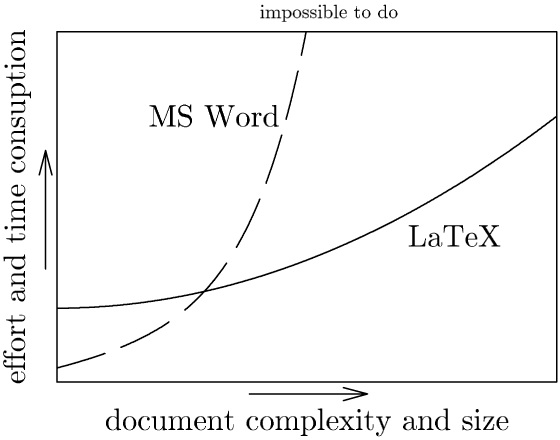
\includegraphics{latex-comparison}
	\caption{Description of the image}
\end{figure}


% This is how we show some code
\begin{verbatim}
<parent>
  <groupId>org.springframework.boot</groupId>
  <artifactId>spring-boot-starter-parent</artifactId>
  <version>3.3.4</version> <!-- bumped version -->
  <relativePath/>
</parent>
\end{verbatim}

\subsubsection{subsubsection}

\begin{itemize}
  \item A
  \item bullet
  \item list
\end{itemize}

\begin{enumerate}
  \item A
  \item numbered
  \item list
\end{enumerate}

\clearpage

\addcontentsline{toc}{section}{References}
\bibliography{refs} % Entries are in the refs.bib file

\end{document}  
